\documentclass[aspectratio=169, 11pt]{beamer}

% --- Packages & Setup ---
\usepackage[utf8]{inputenc}
\usepackage[T1]{fontenc}
\usepackage{helvet}
\renewcommand{\familydefault}{\sfdefault}
\usepackage{xcolor}
\usepackage{booktabs}
\usepackage{array}
\usepackage{graphicx}
\usepackage{amsmath,amssymb}
\usepackage{tikz}
\usetikzlibrary{calc,positioning,arrows.meta,fit,backgrounds}

\graphicspath{{./figures/}{./}}

% --- Branding Colors ---
\definecolor{amritaMaroon}{HTML}{A4123F}
\definecolor{doneGreen}{HTML}{1E7D3A}
\definecolor{todoGrey}{HTML}{8A8A8A}

% --- Theme Setup ---
\usetheme{Madrid}
\usecolortheme[named=amritaMaroon]{structure}
\setbeamertemplate{navigation symbols}{}
\setbeamertemplate{footline}[frame number]

\tikzset{
  stp/.style={draw=amritaMaroon, fill=amritaMaroon!8, rounded corners=2pt, align=center,
              font=\scriptsize, minimum height=1.05cm, text width=1.72cm, inner sep=2pt},
  stpG/.style={stp, draw=doneGreen, fill=doneGreen!8},
  stpT/.style={stp, draw=todoGrey, fill=todoGrey!10, dashed},
  io/.style={draw=black!60, fill=white, rounded corners=2pt, align=center, font=\scriptsize,
             minimum height=0.8cm, text width=2.0cm},
  arr/.style={-{Stealth[length=2mm]}, thick, black!70}
}
\newcommand{\ok}{\textcolor{doneGreen}{\checkmark}}
\newcommand{\no}{\textcolor{amritaMaroon}{$\times$}}

\begin{document}

% =========================================================================
% TITLE SLIDE
% =========================================================================
\begin{frame}
    \begin{tikzpicture}[remember picture,overlay]
        \node[fill=amritaMaroon, text=white, font=\bfseries\footnotesize, anchor=north east, rounded corners=2pt, inner sep=5pt]
        at ($(current page.north east) + (-0.2cm,-0.2cm)$)
        {Type 1: Research Project};
    \end{tikzpicture}

    \centering
    \IfFileExists{logo.png}{
\includegraphics[width=2.8cm]{logo.png}}{\fbox{\footnotesize [logo.png]}}
    \vspace{0.1cm}

    {\large \textbf{\textcolor{amritaMaroon}{MOF Graphs and Crystal Morphology: Crystal Shapes of\\Metal--Organic Frameworks from the Unit Cell}}} \\
    \vspace{0.05cm}
    {\footnotesize \textbf{23CSE498 -- Project Phase II (External Review)} \quad | \quad \textbf{Team Number: G070}} \\
    \vspace{0.15cm}

    \begin{table}
        \centering
        \footnotesize
        \renewcommand{\arraystretch}{1.05}
        \begin{tabular}{|c|c|l|}
            \hline
            \textbf{S.No} & \textbf{Register Number} & \textbf{Student Name} \\
            \hline
            1 & CB.SC.U4CSE23134 & Pasupuleti Meena Radha Krishna \\
            \hline
            2 & CB.SC.U4CSE23122 & Kshitij Varma Pinnamaraju \\
            \hline
            3 & CB.SC.U4CSE23031 & Keerthi Sree Jonnakuti \\
            \hline
            4 & CB.SC.U4CSE23141 & Rohith Abhinav Sai Komal Gullolla \\
            \hline
            5 & CB.SC.U4CSE23029 & Isha Sri Prakash \\
            \hline
        \end{tabular}
    \end{table}
    \vspace{0.1cm}

    {\footnotesize Guide: \textbf{Dr. T. Ramraj}, Assistant Professor (Sl.\ Gd.), Department of CSE} \\
    \vspace{0.1cm}
    {\scriptsize 16 November 2026}
\end{frame}

% =========================================================================
% GUIDE APPROVAL (Mandatory)
% =========================================================================
\begin{frame}{Guide Review \& Submission Approval}
    \framesubtitle{Confirmation of Project Review and Approval from Guide}
    \centering
    \fbox{\begin{minipage}[c][5.4cm]{0.94\textwidth}
        \centering
        \textbf{[Insert Screenshot of Guide Approval Email Here]} \\[0.3cm]
        {\footnotesize [Mandatory: Attach a clear, readable screenshot of the email received from your project guide approving this presentation and final review submission]}
    \end{minipage}}
\end{frame}

\section{Problem \& Solution Design}

% --- SLIDE 1: PROBLEM DEFINITION ---
\begin{frame}[shrink=4]{1. Problem Definition \& Research Motivation}
    \framesubtitle{Problem Statement \& Identified Literature Gap}
    \scriptsize
    \begin{block}{Problem Statement}
        \begin{itemize}
            \item \textbf{Core research problem (panel question after Review 1):} given the unit cell (CIF) of an established MOF, generate the crystal morphologies it can take, mathematically and computationally, and say which one it prefers.
            \item \textbf{Why shape matters:} gas enters a MOF crystal through its faces. At equal volume $V$ the diffusion path is $L = V/A$ and the filling time scales as $L^2$: for $V = 1000\,\mu$m$^3$ a cube has $L = 1.67\,\mu$m, a $20{\times}20{\times}2.5$ plate $1.00\,\mu$m, a $2.5{\times}2.5{\times}160$ needle $0.62\,\mu$m, i.e.\ the needle fills $\approx 7\times$ faster with the same material. Which faces are exposed also decides which pore windows face the gas.
        \end{itemize}
    \end{block}
    \begin{block}{Existing Limitations \& Research Gap}
        \begin{itemize}
            \item \textbf{Existing approaches:} inorganic crystals get surface energies from DFT and shapes from the Wulff construction; MOF slabs have hundreds of atoms, so DFT is too slow for screening. MOF shape work is mostly experimental, one framework and one additive at a time. Machine learning on MOFs targets adsorption and stability, not shape.
            \item \textbf{Gap:} no automated route from an arbitrary MOF CIF to (i) the faces symmetry allows, (ii) chemically sensible surfaces with an energy, (iii) the Wulff shape, (iv) the set of other shapes reachable and how far each is, all checked against laboratory crystals.
        \end{itemize}
    \end{block}
\end{frame}

\begin{frame}[shrink=6]{1. Problem Definition \& Research Motivation (contd.)}
    \framesubtitle{Research Objectives and Status}
    \scriptsize
    \renewcommand{\arraystretch}{1.25}
    \begin{tabular}{>{\raggedright\arraybackslash}p{3.3cm} >{\raggedright\arraybackslash}p{8.1cm} >{\raggedright\arraybackslash}p{2.6cm}}
        \toprule
        \textbf{Objective} & \textbf{What was built and how it was checked} & \textbf{Status} \\
        \midrule
        O1 Faces from symmetry & spglib space group $\rightarrow$ allowed \{hkl\} with exact systematic absences $\rightarrow$ BFDH shape, any lattice; 16 propositions proved; Python and browser engines agree number by number; run on 138 dataset CIFs & \ok\ validated with limits (P1 files) \\
        O2 Energies and Wulff shape & (a) bond-count / UFF cleavage $\gamma$ for cubic MOFs; (b) team pipeline: block-intact slabs, water caps, CHGNet $\gamma$, Wulff & \ok\ main face right for 4 of 5 additive-free MOFs \\
        O3 Validation of $\gamma$ & MACE-MP-0 re-scoring; slab-thickness check; thermodynamic water reference; DFT inputs prepared & \ok\ ranking agrees ($\rho$ 0.94--1.00); DFT not run \\
        O4 Laboratory benchmark & 134 records, 35 papers, 12 MOFs; additive-free vs additive & \ok\ 28/32 records; bootstrap 73--97\% \\
        O5 Fast surrogate & GNN on the slab graph, leave-MOF-out CV against baselines & \ok\ done; does not beat a linear baseline \\
        O6 Shape space & morphology map (exact boundaries) and morphology spectrum (every reachable class + distance) & \ok\ new (spectrum: team notebook v4) \\
        O7 Conditions $\rightarrow$ shape model & laboratory data exist for only 12 MOFs; a held-out-MOF model gets 5/32 & \no\ not feasible yet \\
        \bottomrule
    \end{tabular}
\end{frame}

% --- SLIDE 2: WORKFLOW ---
\begin{frame}{2. Proposed Methodology \& Overall Workflow}
    \framesubtitle{End-to-End Research Methodology / System Workflow Architecture}
    \centering
    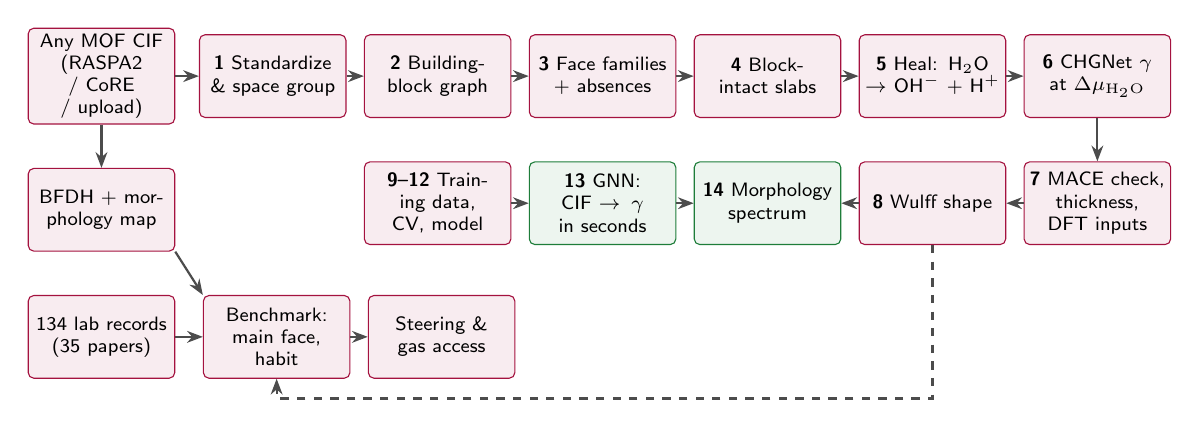
\begin{tikzpicture}[node distance=0.22cm]
        \node[stp] (cif) {Any MOF CIF\\(RASPA2 / CoRE / upload)};
        \node[stp, right=0.3cm of cif] (s1) {\textbf{1} Standardize \& space group};
        \node[stp, right=of s1] (s2) {\textbf{2} Building-block graph};
        \node[stp, right=of s2] (s3) {\textbf{3} Face families + absences};
        \node[stp, right=of s3] (s4) {\textbf{4} Block-intact slabs};
        \node[stp, right=of s4] (s5) {\textbf{5} Heal: H$_2$O $\rightarrow$ OH$^-$ + H$^+$};
        \node[stp, right=of s5] (s6) {\textbf{6} CHGNet $\gamma$ at $\Delta\mu_{\mathrm{H_2O}}$};

        \node[stp, below=0.55cm of s6] (s7) {\textbf{7} MACE check, thickness, DFT inputs};
        \node[stp, left=of s7] (s8) {\textbf{8} Wulff shape};
        \node[stpG, left=of s8] (s14) {\textbf{14} Morphology spectrum};
        \node[stpG, left=of s14] (s13) {\textbf{13} GNN: CIF $\rightarrow\gamma$ in seconds};
        \node[stp, left=of s13] (s912) {\textbf{9--12} Training data, CV, model};

        \node[stp, below=0.55cm of cif] (bf) {BFDH + morphology map};
        \node[stp, below=0.55cm of bf] (lab) {134 lab records (35 papers)};
        \node[stp, right=0.35cm of lab] (bench) {Benchmark: main face, habit};
        \node[stp, right=of bench] (steer) {Steering \& gas access};

        \draw[arr] (cif) -- (s1); \draw[arr] (s1) -- (s2); \draw[arr] (s2) -- (s3);
        \draw[arr] (s3) -- (s4); \draw[arr] (s4) -- (s5); \draw[arr] (s5) -- (s6);
        \draw[arr] (s6) -- (s7); \draw[arr] (s7) -- (s8); \draw[arr] (s8) -- (s14);
        \draw[arr] (s912) -- (s13); \draw[arr] (s13) -- (s14);
        \draw[arr] (cif) -- (bf); \draw[arr] (lab) -- (bench); \draw[arr] (bench) -- (steer);
        \draw[arr] (bf.south east) -- (bench.north west);
        \draw[arr, dashed] (s8.south) |- ($(bench.south)+(0,-0.25)$) -- (bench.south);
    \end{tikzpicture}
    \vspace{0.1cm}

    \begin{block}{Workflow Summary}
        \scriptsize Track A (left): symmetry $\rightarrow$ allowed faces $\rightarrow$ BFDH $\rightarrow$ map, in seconds for any CIF. Track B (top): steps 1--8 turn a CIF into per-face surface energies $\gamma_{hkl}$ and a Wulff shape; steps 9--13 train a GNN that replaces the slow relaxation; step 14 (green, new in notebook v4) lists every shape the faces can make and how far each is. Both tracks are scored against laboratory crystals.
    \end{block}
\end{frame}

% --- SLIDE 3: FORMULATION ---
\begin{frame}[shrink=10]{3. Methodological Components \& Formulation}
    \framesubtitle{Governing Mathematical Model (1/2): faces and shapes}
    \begin{columns}[T]
        \column{0.50\textwidth}
        \begin{block}{Allowed faces from the space group}
            \scriptsize
            \begin{itemize}
                \item Plane spacing: $\displaystyle d_{hkl} = \frac{1}{\lVert h\,G^{-1}\rVert}$; cubic: $d_{hkl} = \dfrac{a}{\sqrt{h^2+k^2+l^2}}$.
                \item Exact absence: reflection $n\,h$ is extinct if some operation $(R,t)$ has $hR = h$ and $h\cdot t \notin \mathbb{Z}$. First allowed order $n$ gives $d_\text{eff} = d_{hkl}/n$.
                \item Centring: I needs $h{+}k{+}l$ even; F needs $h,k,l$ all even or all odd. ZIF-8 (I-43m, $a = 16.99$\,\AA): $d_\text{eff}$\{110\} 12.0, \{100\} 8.5, \{111\} 4.9\,\AA\ $\Rightarrow$ rhombic dodecahedron.
                \item BFDH: face distance $\propto 1/d_\text{eff}$; F-cubic gives $\{111\}:\{100\} = 1 : 1.155$ $\Rightarrow$ truncated octahedron (78\% \{111\}).
            \end{itemize}
        \end{block}
        \column{0.47\textwidth}
        \begin{block}{Wulff construction and the cubic map}
            \scriptsize
            \begin{itemize}
                \item Minimise $\sum_i \gamma_i A_i$ at fixed $V$ $\Rightarrow$ $W = \{x : \hat n_i\cdot x \le \gamma_i\ \forall i\}$ (half-space intersection; an LP detects open shapes).
                \item Shape depends only on ratios: $x = \gamma_{110}/\gamma_{100}$, $y = \gamma_{111}/\gamma_{100}$.
                \item Exact boundaries: cube $y \ge \sqrt3$ and $x \ge \sqrt2$; octahedron $y \le 1/\sqrt3$; cuboctahedron $y = 2/\sqrt3$.
                \item Attachment number on the net (bonds a new node makes): pcu \{100\},\{110\},\{111\} = 1,2,3 $\Rightarrow$ cube; fcu \{111\},\{100\},\{110\} = 3,4,5 $\Rightarrow$ octahedron.
                \item Cell stretch $c \rightarrow \lambda c$: height/width $= 1/\lambda$ (box law) for $\lambda \gtrsim 0.8$.
            \end{itemize}
        \end{block}
    \end{columns}
\end{frame}

\begin{frame}[shrink=10]{3. Methodological Components \& Formulation (contd.)}
    \framesubtitle{Governing Mathematical Model (2/2): surface energy, water, spectrum, GNN}
    \begin{columns}[T]
        \column{0.52\textwidth}
        \begin{block}{Surface energy with a water reservoir}
            \scriptsize
            \[ \gamma = \frac{E_\text{slab} - N e_\text{bulk} - n\,\mu_{\mathrm{H_2O}}}{2A}, \quad 1\ \text{eV/\AA}^2 = 16.02\ \text{J/m}^2 \]
            \[ \gamma(\Delta\mu) = \gamma_{0\,\mathrm K} - \frac{n\,\Delta\mu}{2A} \]
            $N$ formula units, $n$ water caps, $A$ area of one face. $\Delta\mu$ from NIST-JANAF / CODATA: vapour 298\,K 1\,bar $-0.481$; \textbf{liquid 298\,K $-0.570$}; 50\% RH $-0.587$; 400\,K $-0.686$\,eV (ZPE omitted, $\pm0.1$\,eV).
        \end{block}
        \begin{block}{Bond-count energy}
            \scriptsize $\gamma \approx \dfrac{\sum_\text{cut} \varepsilon_b}{2A}$ with UFF pair energies; 93--98\% of $\gamma$ is the broken-bond term.
        \end{block}
        \column{0.45\textwidth}
        \begin{block}{Morphology spectrum (notebook v4)}
            \scriptsize
            Distance from the favoured energies $g_0$ to $g$:
            \[ s = \max_k \ln\frac{g_k}{g_{0,k}} - \min_k \ln\frac{g_k}{g_{0,k}}, \quad \Delta = (e^{s}-1)\times100\% \]
            Scale-free and independent of the reference face. Scan: grid 0.3--2.5, step 0.05 (cubic, 2\,025 shapes) or Sobol \cite{sobol1967} (4 faces); closest point of each class refined by bisection along $\ln g$, then re-checked.
        \end{block}
        \begin{block}{GNN surrogate}
            \scriptsize Message passing \cite{gilmer2017} on the atom graph of the unrelaxed healed slab $\rightarrow$ softplus $\rightarrow\gamma$; loss = Huber($\delta$=0.3) + 0.5 $\times$ pairwise rank loss within each MOF; pretrained on static $\gamma$; leave-MOF-out CV.
        \end{block}
    \end{columns}
\end{frame}

\begin{frame}[shrink=6]{3. Methodological Components \& Formulation (contd.)}
    \framesubtitle{Datasets, Partitioning \& Evaluation Metrics}
    \begin{columns}[T]
        \column{0.5\textwidth}
        \begin{block}{Dataset \& Input Specifications}
            \scriptsize
            \begin{itemize}
                \item \textbf{Structures:} 138 dataset CIFs (77 hMOF, 61 CoRE MOF); RASPA2 library (105 readable CIFs; 16 MOFs relaxed, 41 static for pretraining).
                \item \textbf{Laboratory morphology:} 134 records, 35 papers, 12 MOFs, each with additive, solvent, temperature, habit, faces and source locator.
                \item \textbf{Preprocessing:} disorder (majority), guest removal, overlap merge; symmetry retried on the H-free skeleton (ZIF-8 is P1 with H, I-43m without).
            \end{itemize}
        \end{block}
        \column{0.46\textwidth}
        \begin{block}{Partitioning \& Metrics}
            \scriptsize
            \begin{itemize}
                \item \textbf{Main face / habit accuracy} against records; baseline = per-MOF lab majority with the paper held out; bootstrap over whole papers.
                \item \textbf{GNN:} leave-one-MOF-out (16 folds); MAE (J/m$^2$), Spearman of face order, lowest face right, main face right.
                \item \textbf{CHGNet vs MACE:} Spearman $\rho$ and MAE of $\gamma$.
                \item \textbf{Spectrum:} distance $\Delta$ to the laboratory class.
            \end{itemize}
        \end{block}
    \end{columns}
\end{frame}

% =========================================================================
% SECTION 2: IMPLEMENTATION
% =========================================================================
\section{Implementation Details}

\begin{frame}[shrink=4]{4. Implementation Details -- Overview}
    \framesubtitle{Module-Wise Implementation \& Pipeline Integration}
    \begin{table}
        \centering
        \scriptsize
        \renewcommand{\arraystretch}{1.18}
        \begin{tabular}{>{\raggedright\arraybackslash}p{3.0cm} >{\raggedright\arraybackslash}p{11.4cm}}
            \toprule
            \textbf{Module / Stage} & \textbf{Functionality} \\
            \midrule
            1. Standardization & Reads a CIF (RASPA2 URL, CoRE MOF refcode, upload); resolves partial occupancy, removes guests, merges overlapping sites; spglib space group with fallback to the H-free or metal--carbon skeleton. \\
            2. Building blocks & Bond graph labels pairs organic, metal--metal, metal--oxo, metal--ligand; components without metal--ligand edges are nodes and linkers; periodic rods found from lattice-image offsets. \\
            3. Face families & Miller indices to \texttt{max\_index}, grouped by $h' = hR^{-1}$ (+ inversion), ranked by $d_\text{eff}$ with exact absences; keep the top $N$ (= 4). \\
            4. Slab construction & Block centroids projected on $\hat n$, grouped into layers; one termination per inter-layer gap; 15\,\AA\ slab, 15\,\AA\ vacuum; whole formula units asserted; broken bonds per area counted. \\
            5. Surface healing & Each exposed metal gets OH (2.0\,\AA), the donor O gets H (0.98\,\AA) along the most open direction on a Fibonacci sphere; clashes or broken organic bonds reject the slab. \\
            \bottomrule
        \end{tabular}
    \end{table}
\end{frame}

\begin{frame}[shrink=6]{4. Implementation Details -- Overview (contd.)}
    \framesubtitle{Module-Wise Implementation \& Pipeline Integration}
    \begin{table}
        \centering
        \scriptsize
        \renewcommand{\arraystretch}{1.18}
        \begin{tabular}{>{\raggedright\arraybackslash}p{3.0cm} >{\raggedright\arraybackslash}p{11.4cm}}
            \toprule
            \textbf{Module / Stage} & \textbf{Functionality} \\
            \midrule
            6. Surface energy & CHGNet static screen of all terminations, relaxation of the best $K$ (= 2) to $F_\text{max} < 0.05$ eV/\AA\ (800 steps); $\gamma$ from slab, bulk and water energies; cached per slab. \\
            7. Validation & MACE-MP-0 re-scores bulk, water and slabs on the CHGNet geometries; thicker-slab check; CP2K PBE-D3 inputs (normal along $z$, dipole correction). \\
            8. Wulff morphology & Lowest converged $\gamma$ per family $\rightarrow$ half-space intersection $\rightarrow$ area fractions, habit name, image and OBJ mesh. \\
            9--13. GNN surrogate & RASPA2 survey for training slabs; graphs exported per slab; leave-MOF-out CV vs five baselines; final model saved; new CIF $\rightarrow$ $\gamma$ $\rightarrow$ Wulff without CHGNet. \\
            14. Morphology spectrum & \texttt{morphspec.py}: favoured shape + every shape class with its distance; self-tests (14a), one CIF (14b), all computed MOFs (14c). \\
            Track A, website & \texttt{mofmorph/} (Python) and browser engines; 28 pages built from fragments; 15 jsdom test suites. \\
            \bottomrule
        \end{tabular}
    \end{table}
    \begin{block}{Implementation Environment \& Repository}
        \scriptsize Python (pymatgen, spglib, ASE, networkx, SciPy HalfspaceIntersection/linprog/Sobol, PyTorch), CHGNet and MACE-MP-0 on a Colab GPU; JavaScript engines for the website. Final team notebook: \texttt{MOF\_Wulff\_steps1-8\_plus\_GNN\_v4.ipynb}. Repository: \texttt{github.com/Radha-Krishna-19/fyp}.
    \end{block}
\end{frame}

\begin{frame}[shrink=10]{5. Core Module Implementation Details}
    \framesubtitle{Internal Module Mechanics, Parameter Configurations \& Interfaces}
    \begin{columns}[T]
        \column{0.50\textwidth}
        \begin{block}{Slab builder \& healer (\texttt{block\_slabs}, \texttt{heal})}
            \scriptsize
            \begin{itemize}
                \item \textbf{In/Out:} conventional cell + (hkl) $\rightarrow$ terminations (slab, broken-bond counts, $n$ caps).
                \item \textbf{Rule:} cut only metal--ligand bonds; a bridging O that loses two bonds may receive at most one H (otherwise C--OH$_2^+$ appears: 26 of 118 slabs under the old rule).
                \item \textbf{Parameters:} thickness 15\,\AA, vacuum 15\,\AA, \texttt{level\_tol} 0.3\,\AA, \texttt{max\_terms} 8, M--X 2.55\,\AA, M--M 2.80\,\AA.
            \end{itemize}
        \end{block}
        \begin{block}{Spectrum (\texttt{morphspec.scan\_morphology\_map})}
            \scriptsize
            \begin{itemize}
                \item \textbf{In:} conv lattice, families, rotations, $\gamma_0$, BFDH point. \textbf{Out:} classes, distances, map, Wulff images.
                \item Class = habit name + faces with area $\ge 5\%$; bisection 12 steps; cache keyed on rounded ratios.
            \end{itemize}
        \end{block}
        \column{0.46\textwidth}
        \centering
        \vspace{0.1cm}
        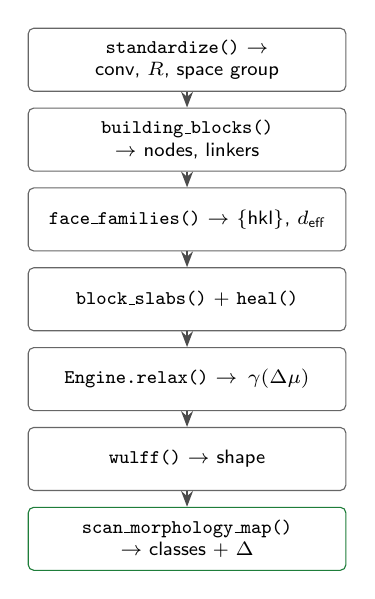
\begin{tikzpicture}[node distance=0.2cm, every node/.style={font=\scriptsize}]
            \node[io, text width=3.8cm] (a) {\texttt{standardize()} $\rightarrow$ conv, $R$, space group};
            \node[io, text width=3.8cm, below=of a] (b) {\texttt{building\_blocks()} $\rightarrow$ nodes, linkers};
            \node[io, text width=3.8cm, below=of b] (c) {\texttt{face\_families()} $\rightarrow$ \{hkl\}, $d_\text{eff}$};
            \node[io, text width=3.8cm, below=of c] (d) {\texttt{block\_slabs()} + \texttt{heal()}};
            \node[io, text width=3.8cm, below=of d] (e) {\texttt{Engine.relax()} $\rightarrow \gamma(\Delta\mu)$};
            \node[io, text width=3.8cm, below=of e] (f) {\texttt{wulff()} $\rightarrow$ shape};
            \node[io, text width=3.8cm, below=of f, draw=doneGreen] (g) {\texttt{scan\_morphology\_map()} $\rightarrow$ classes + $\Delta$};
            \foreach \x/\y in {a/b,b/c,c/d,d/e,e/f,f/g} \draw[arr] (\x) -- (\y);
        \end{tikzpicture}
    \end{columns}
\end{frame}

% =========================================================================
% SECTION 3: VERIFICATION
% =========================================================================
\section{Verification \& Demonstration}

\begin{frame}[shrink=4]{6. Experimental Visualizations \& Prototype Demonstration}
    \framesubtitle{Structure-only models against 134 laboratory records}
    \begin{columns}[c]
        \column{0.52\textwidth}
        \centering
        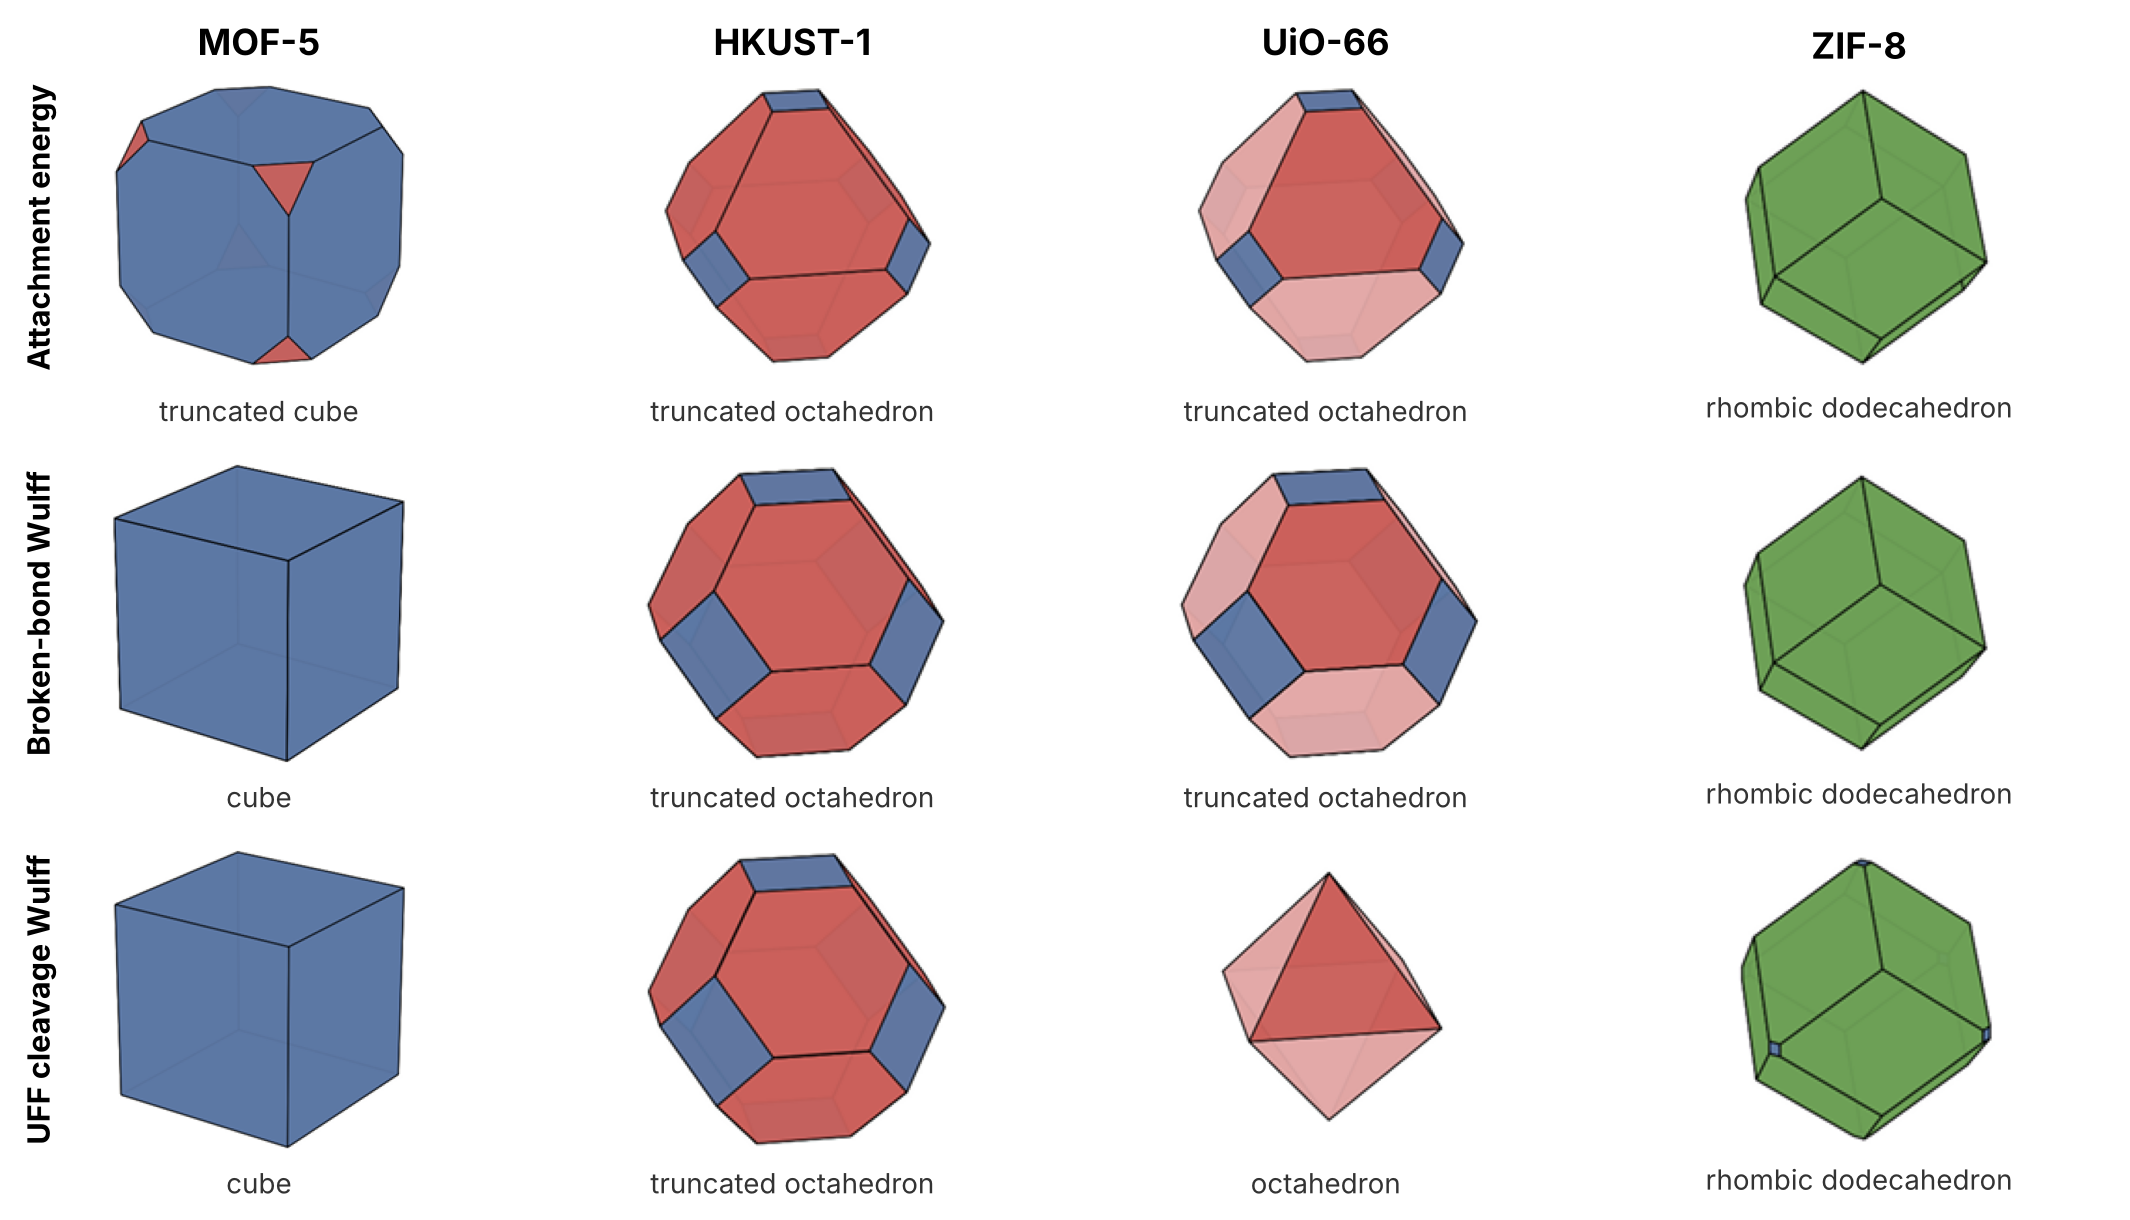
\includegraphics[width=\textwidth]{morphology_grid.png}\\
        {\tiny Predicted habits of four MOFs from three surface models.}
        \column{0.46\textwidth}
        \scriptsize
        \renewcommand{\arraystretch}{1.2}
        \begin{tabular}{lccc}
            \toprule
            \textbf{Main face} & \textbf{No add.} & \textbf{Add.} & \textbf{All} \\
            & (32) & (44) & (76) \\
            \midrule
            BFDH & 56\% & 48\% & 51\% \\
            Bond-count Wulff & \textbf{88\%} & 39\% & 59\% \\
            Lab majority, paper out & 88\% & 30\% & 54\% \\
            Other MOFs, MOF out & 16\% & 39\% & 29\% \\
            \bottomrule
        \end{tabular}\\[0.15cm]
        \begin{itemize}
            \item Additive-free: MOF-5 9/9, ZIF-8 11/12, HKUST-1 7/8, IRMOF-3 1/1, UiO-66 0/2 $\Rightarrow$ 4 of 5 MOFs; paper bootstrap 73--97\%.
            \item Habit: BFDH 85/97 vs 76 for ``always compact''; predicts the Mg-MOF-74 rods (9 of 10 lab crystals elongated).
            \item With additives no structure-only model is reliable.
        \end{itemize}
    \end{columns}
\end{frame}

\begin{frame}[shrink=4]{6. Experimental Visualizations \& Prototype Demonstration (contd.)}
    \framesubtitle{The space of shapes: one exact map and one family}
    \begin{columns}[c]
        \column{0.40\textwidth}
        \centering
        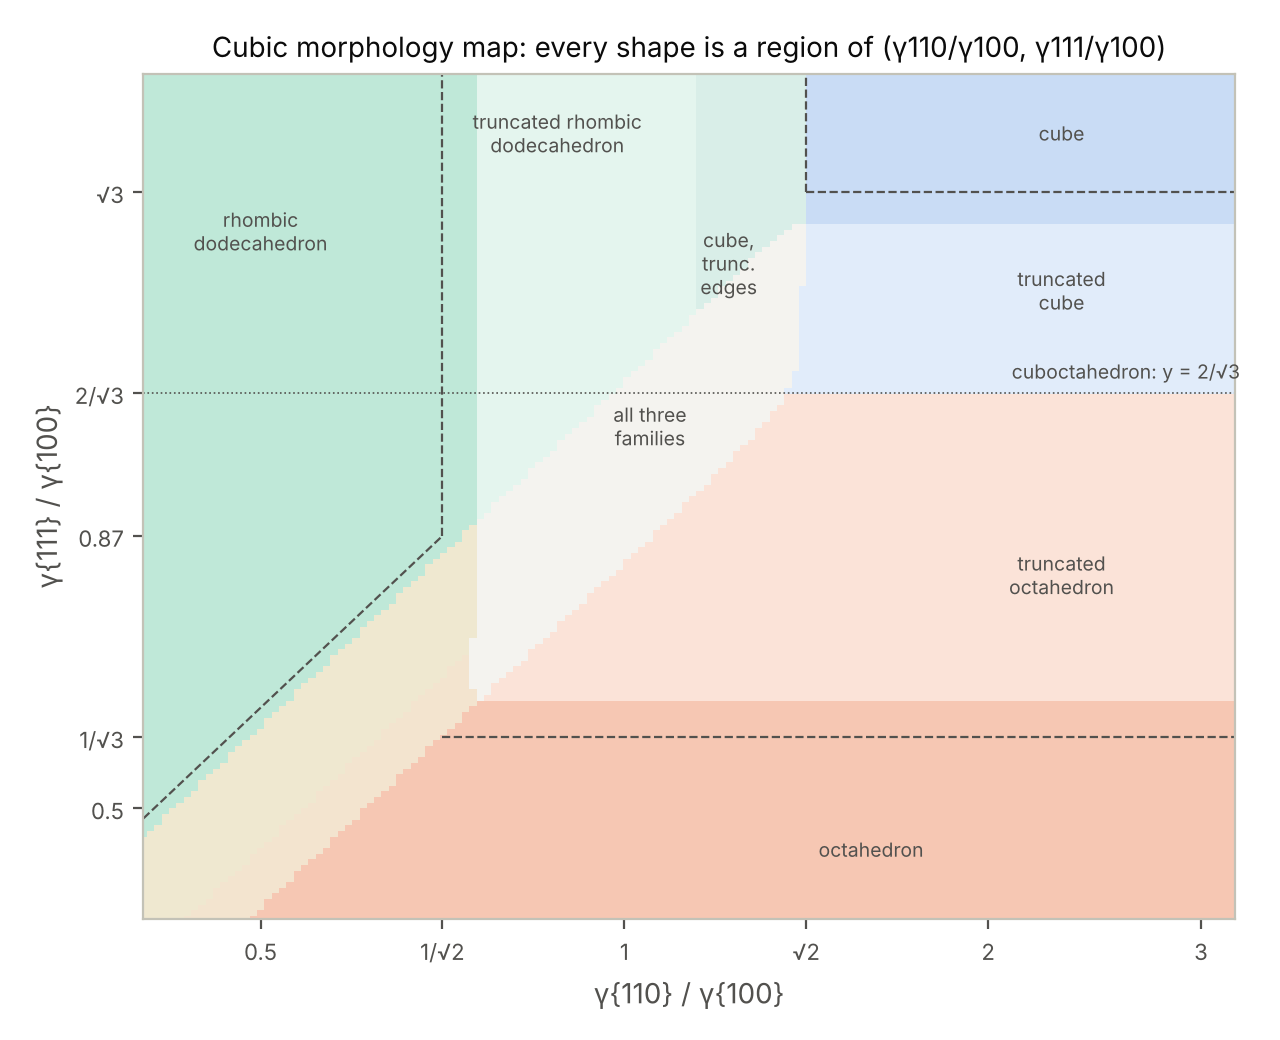
\includegraphics[width=\textwidth]{map_regions.png}
        \column{0.58\textwidth}
        \centering
        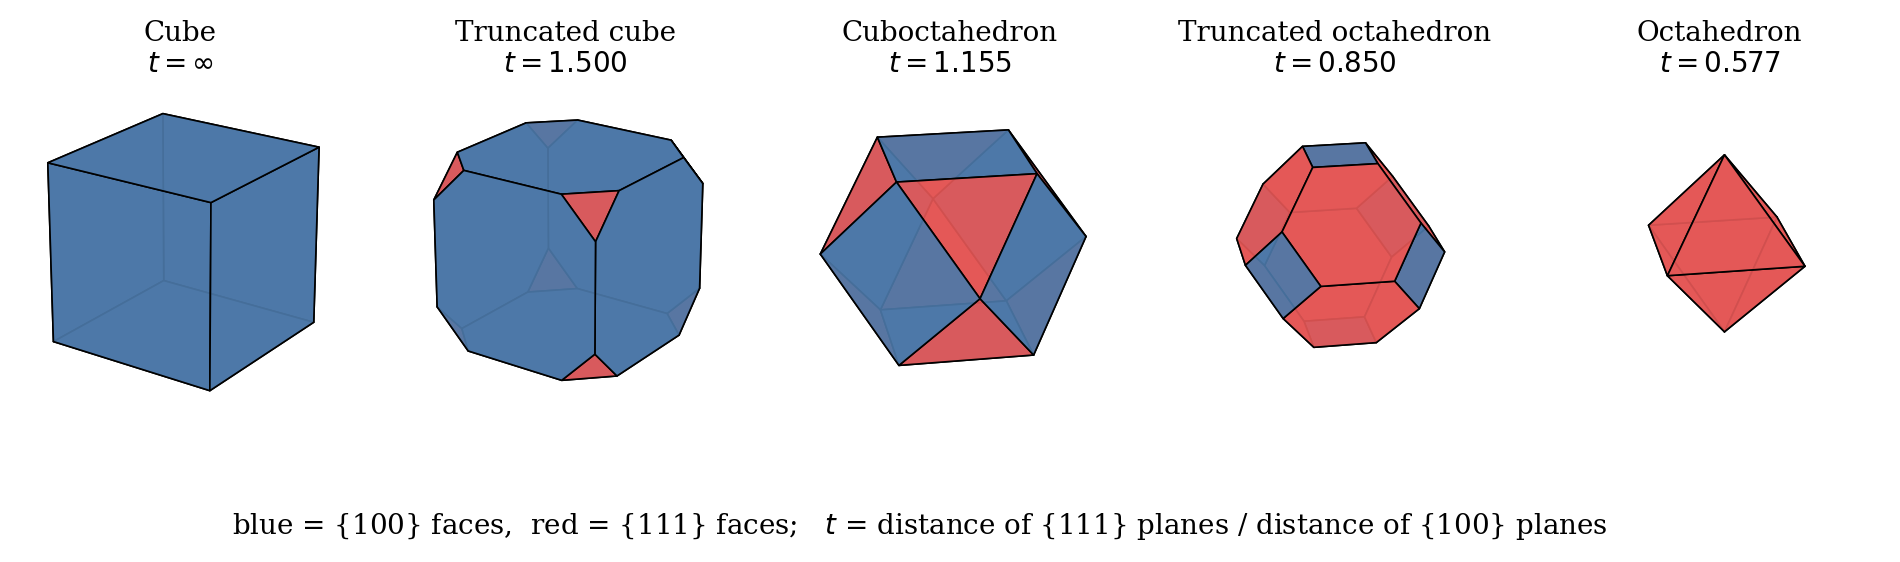
\includegraphics[height=1.55cm]{morph_path.png}\\[0.05cm]
        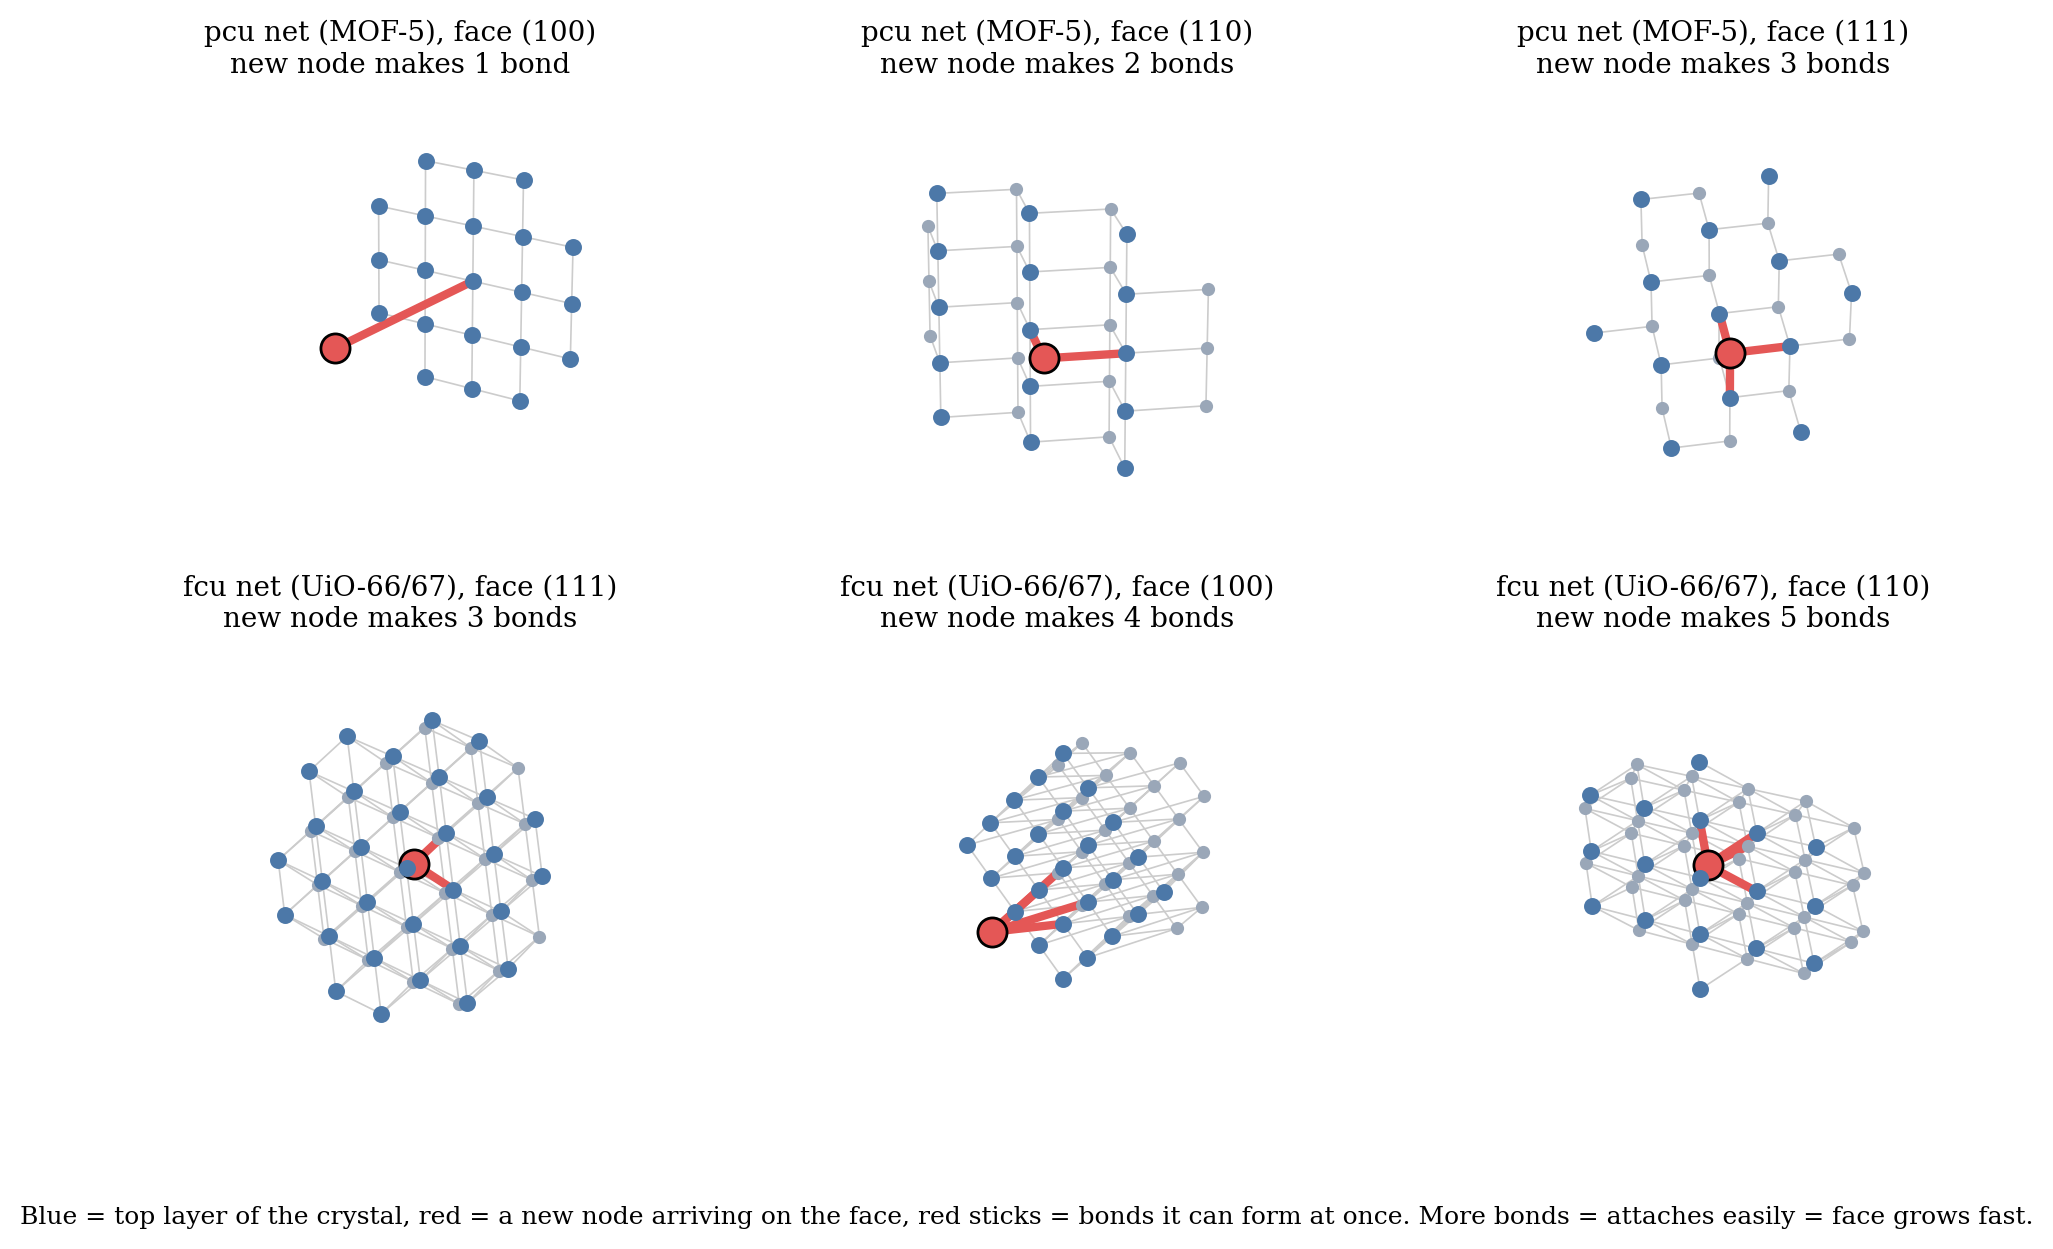
\includegraphics[height=2.6cm]{attach.png}\\
        \scriptsize
        \begin{itemize}
            \item Top: $t = d_{111}/d_{100}$ from $\infty$ (cube) via $2/\sqrt3$ (cuboctahedron) to $1/\sqrt3$ (octahedron).
            \item Bottom: attachment numbers on the coarse net explain MOF-5 cubes and UiO-66 octahedra.
            \item MOF-5: $x = 2.81$, $y = 1.73$ (cube); \{111\} must fall 38.1\% to dominate, 66.6\% for an octahedron.
        \end{itemize}
    \end{columns}
\end{frame}

\begin{frame}[shrink=4]{6. Experimental Visualizations \& Prototype Demonstration (contd.)}
    \framesubtitle{Machine-learned energies: why six $\gamma$ were negative, and the correction}
    \centering
    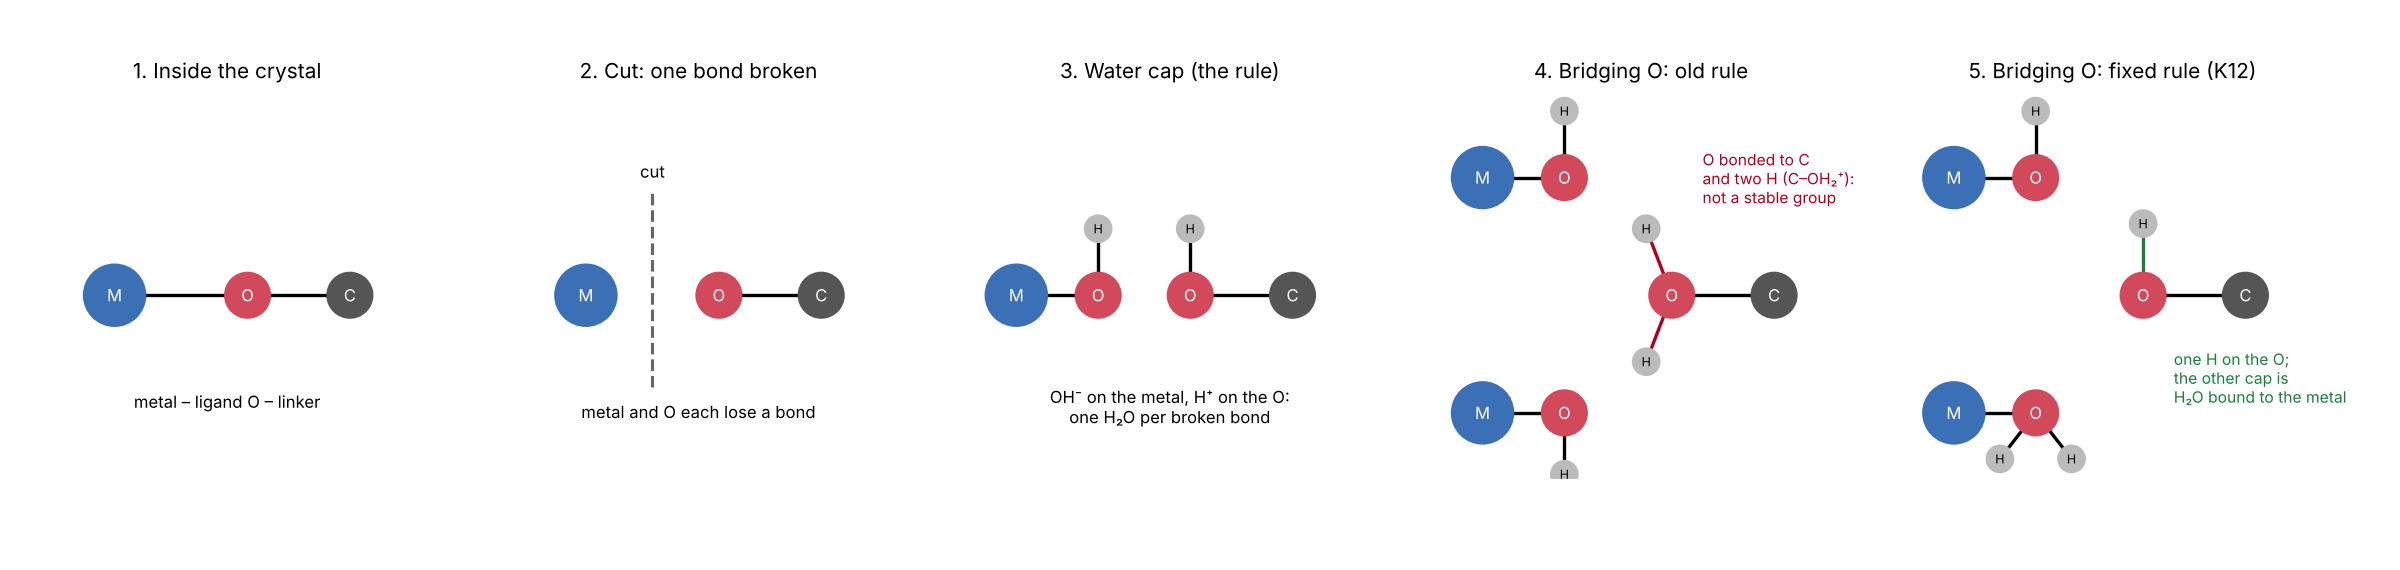
\includegraphics[height=2.2cm]{capping.png}\\[0.05cm]
    \begin{columns}[c]
        \column{0.46\textwidth}
        \centering
        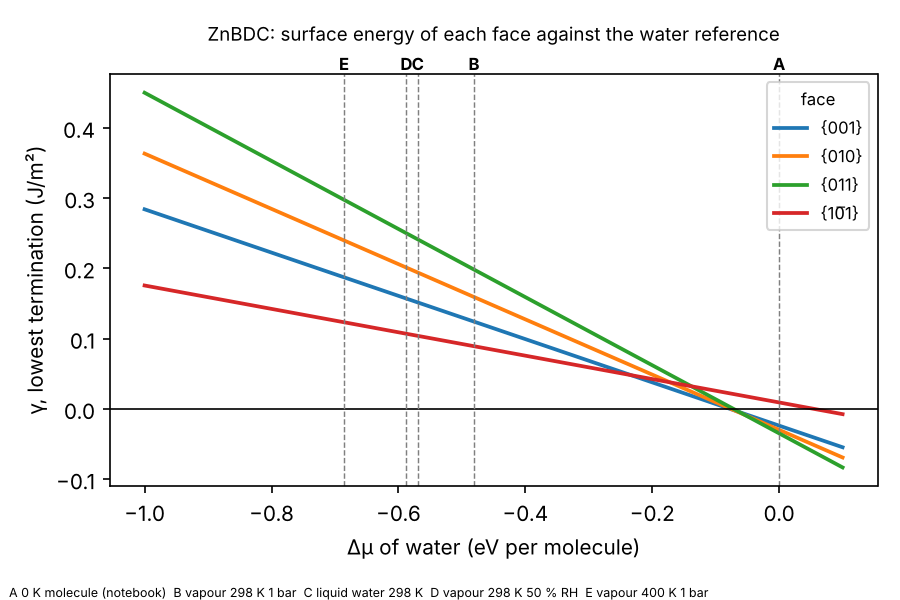
\includegraphics[height=3.4cm]{gamma_mu_ZnBDC.png}
        \column{0.52\textwidth}
        \scriptsize
        \begin{itemize}
            \item Cut M--O bonds are capped with water split into OH$^-$ + H$^+$. The 14 Nov notebook priced each water at a free molecule at 0\,K, the cheapest it can ever be, so capping looked like pure gain.
            \item ZnBDC \{001\}: $n = 4$, $A = 104.08$\,\AA$^2$ $\Rightarrow$ $n/2A = 0.308$\,J/m$^2$ per eV; $\gamma = -0.024 + 0.308\times0.5695 = +0.151$\,J/m$^2$ at liquid water.
            \item Also fixed: at most one H per donor O; Mg--O rod kept whole; relaxed-cell slabs; hydroxylated UiO-66 input; exact face ranking; shape names; DFT input geometry.
        \end{itemize}
    \end{columns}
\end{frame}

\begin{frame}[shrink=4]{6. Experimental Visualizations \& Prototype Demonstration (contd.)}
    \framesubtitle{Corrected GPU run (15 Nov): 98 relaxed slabs, 16 MOFs, liquid water}
    \centering
    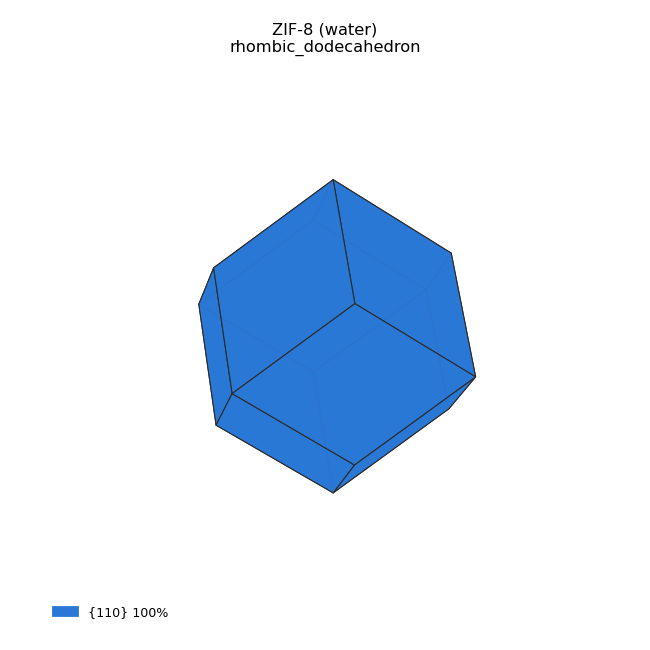
\includegraphics[height=2.6cm]{wulff_ZIF8.png}\hspace{0.1cm}
    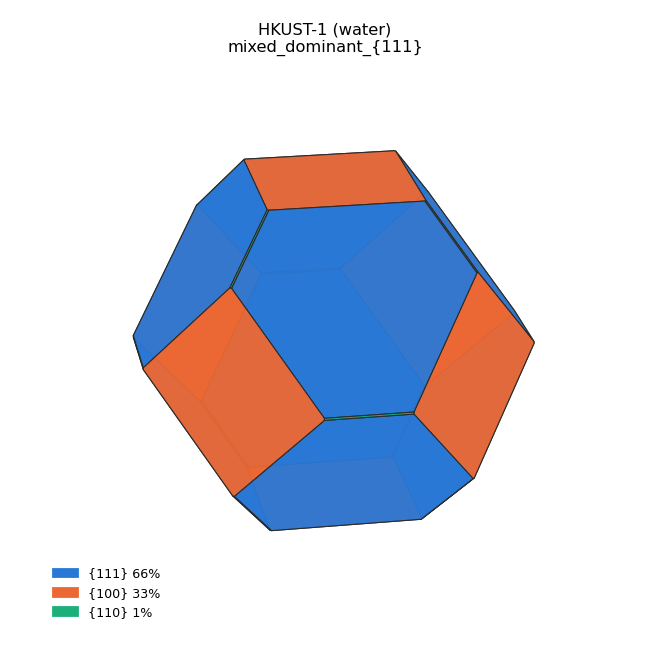
\includegraphics[height=2.6cm]{wulff_HKUST1.png}\hspace{0.1cm}
    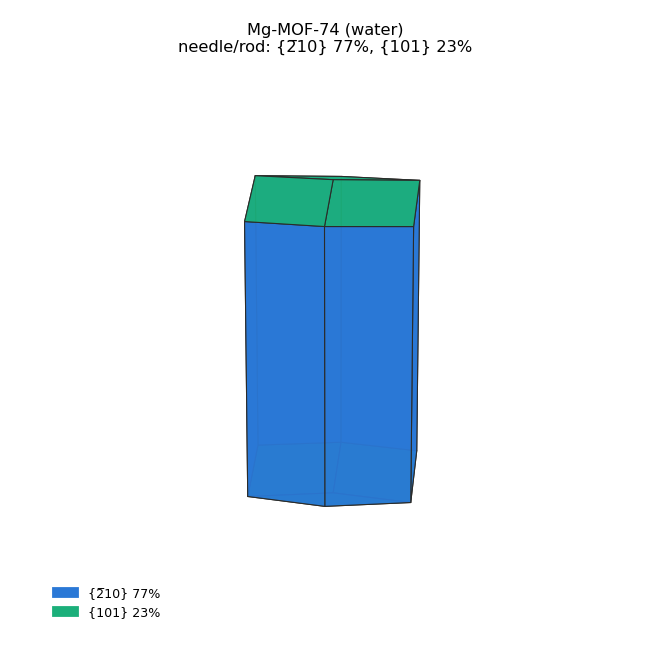
\includegraphics[height=2.6cm]{wulff_MgMOF74.png}\hspace{0.1cm}
    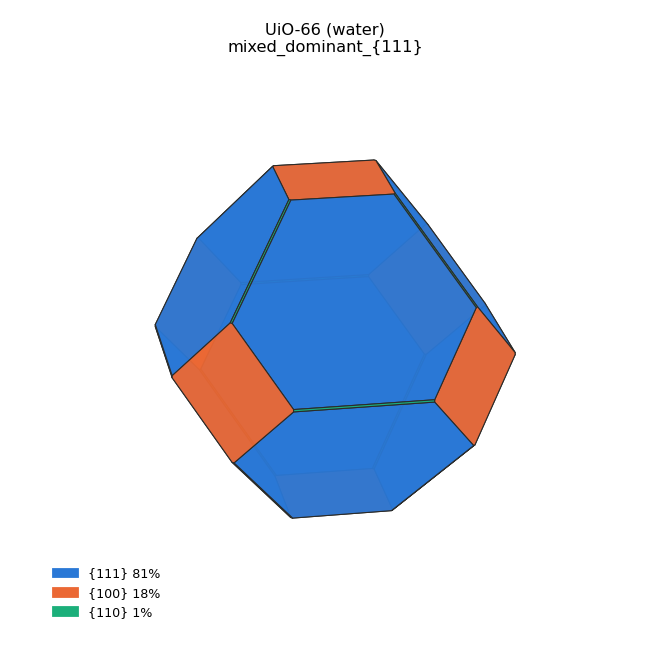
\includegraphics[height=2.6cm]{wulff_UiO66.png}\\[0.1cm]
    \scriptsize
    \renewcommand{\arraystretch}{1.12}
    \begin{tabular}{llll}
        \toprule
        \textbf{MOF} & \textbf{Before (14 Nov)} & \textbf{Corrected, liquid water} & \textbf{Laboratory} \\
        \midrule
        ZIF-8 & rhombic dodecahedron & \{110\} 100\% & rhombic dodecahedron \ok \\
        HKUST-1 & truncated octahedron & \{111\} 66\%, \{100\} 33\% & octahedron \{111\} \ok\ (main face) \\
        Mg-MOF-74 & no shape ($\gamma < 0$) & hexagonal rod, \{2$\bar1$0\} 77\%, \{101\} 23\% & rods along $c$ \ok \\
        UiO-66 & truncated octahedron & \{111\} 81\%, \{100\} 18\% & cube without additives \no \\
        \bottomrule
    \end{tabular}\\[0.1cm]
    85 of 98 converged; 6 negative at 0\,K, \textbf{none at liquid water}; ZIF-8 \{110\} at 24 vs 36\,\AA: $\gamma$ 0.0565 vs 0.0527\,J/m$^2$; MACE-MP-0 vs CHGNet: Spearman 0.94--1.00, MAE 0.010--0.028\,J/m$^2$.
\end{frame}

\begin{frame}[shrink=4]{6. Experimental Visualizations \& Prototype Demonstration (contd.)}
    \framesubtitle{GNN surrogate: leave-one-MOF-out cross-validation (16 MOFs, corrected labels)}
    \begin{columns}[c]
        \column{0.56\textwidth}
        \scriptsize
        \renewcommand{\arraystretch}{1.2}
        \begin{tabular}{lcccc}
            \toprule
            \textbf{Model} & \textbf{MAE} & \textbf{Spearman} & \textbf{Lowest} & \textbf{Main} \\
            & J/m$^2$ & faces & face & face \\
            \midrule
            Static CHGNet, rescaled & \textbf{0.084} & 0.68 & 0.69 & 0.75 \\
            Line on bonds/area & 0.088 & 0.68 & 0.63 & \textbf{0.88} \\
            \textbf{GNN} & 0.131 & 0.45 & 0.50 & 0.75 \\
            Mean & 0.146 & -- & 0.19 & 0.31 \\
            Line on BFDH & 0.150 & $-0.44$ & 0.19 & 0.38 \\
            Static CHGNet & 0.542 & 0.68 & 0.69 & 0.75 \\
            \bottomrule
        \end{tabular}
        \column{0.42\textwidth}
        \scriptsize
        \begin{block}{Reading}
            \begin{itemize}
                \item The GNN (built by Isha) predicts relaxed $\gamma$ from the unrelaxed slab in seconds, against minutes of CHGNet relaxation.
                \item It is behind two one-parameter baselines: broken bonds per area already carry most of $\gamma$ (93--98\% in the bond-count model).
                \item 16 MOFs is small; differences of a few hundredths are within seed spread. Learning target is CHGNet, not experiment.
            \end{itemize}
        \end{block}
    \end{columns}
\end{frame}

\begin{frame}[shrink=4]{6. Experimental Visualizations \& Prototype Demonstration (contd.)}
    \framesubtitle{Morphology spectrum on the corrected energies: how far is the laboratory shape?}
    \begin{columns}[c]
        \column{0.50\textwidth}
        \centering
        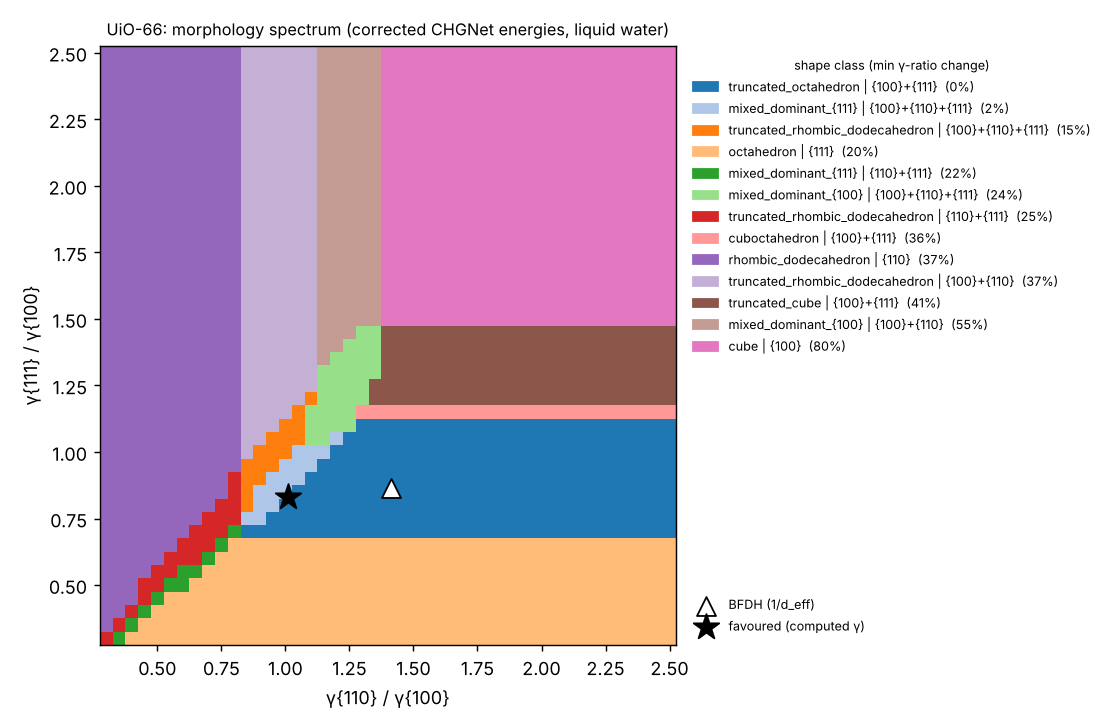
\includegraphics[width=\textwidth]{spec_map_UiO66.png}
        \column{0.48\textwidth}
        \scriptsize
        \renewcommand{\arraystretch}{1.15}
        \begin{tabular}{p{1.3cm}p{1.9cm}p{2.6cm}}
            \toprule
            \textbf{MOF} & \textbf{Favoured} & \textbf{Distance to lab shape} \\
            \midrule
            ZIF-8 & rh.\ dodecahedron & 0\% (same class) \\
            Mg-MOF-74 & hexagonal rod & 0\% (same class) \\
            HKUST-1 & trunc.\ octahedron & octahedron 37.2\% \\
            UiO-66 & trunc.\ octahedron & octahedron (with acid) 19.7\%; cube (no additive) 80.4\% \\
            \bottomrule
        \end{tabular}\\[0.1cm]
        \begin{itemize}
            \item Star = computed energies, triangle = BFDH. 13 shape classes for each cubic MOF, 27 for Mg-MOF-74.
            \item ``Octahedron'' = $\ge$95\% \{111\}; a perfect octahedron needs $\gamma_{111}/\gamma_{100} = 1/\sqrt3$ (43.7\% for UiO-66).
            \item An additive binding \{111\} moves UiO-66 the observed way; the additive-free cube stays unexplained.
        \end{itemize}
    \end{columns}
\end{frame}

\begin{frame}[shrink=2]{6. Experimental Visualizations \& Prototype Demonstration (contd.)}
    \framesubtitle{Morphology spectrum of MIL-125 (team run of notebook v4, by Isha)}
    \centering
    \begin{minipage}{0.30\textwidth}\centering
        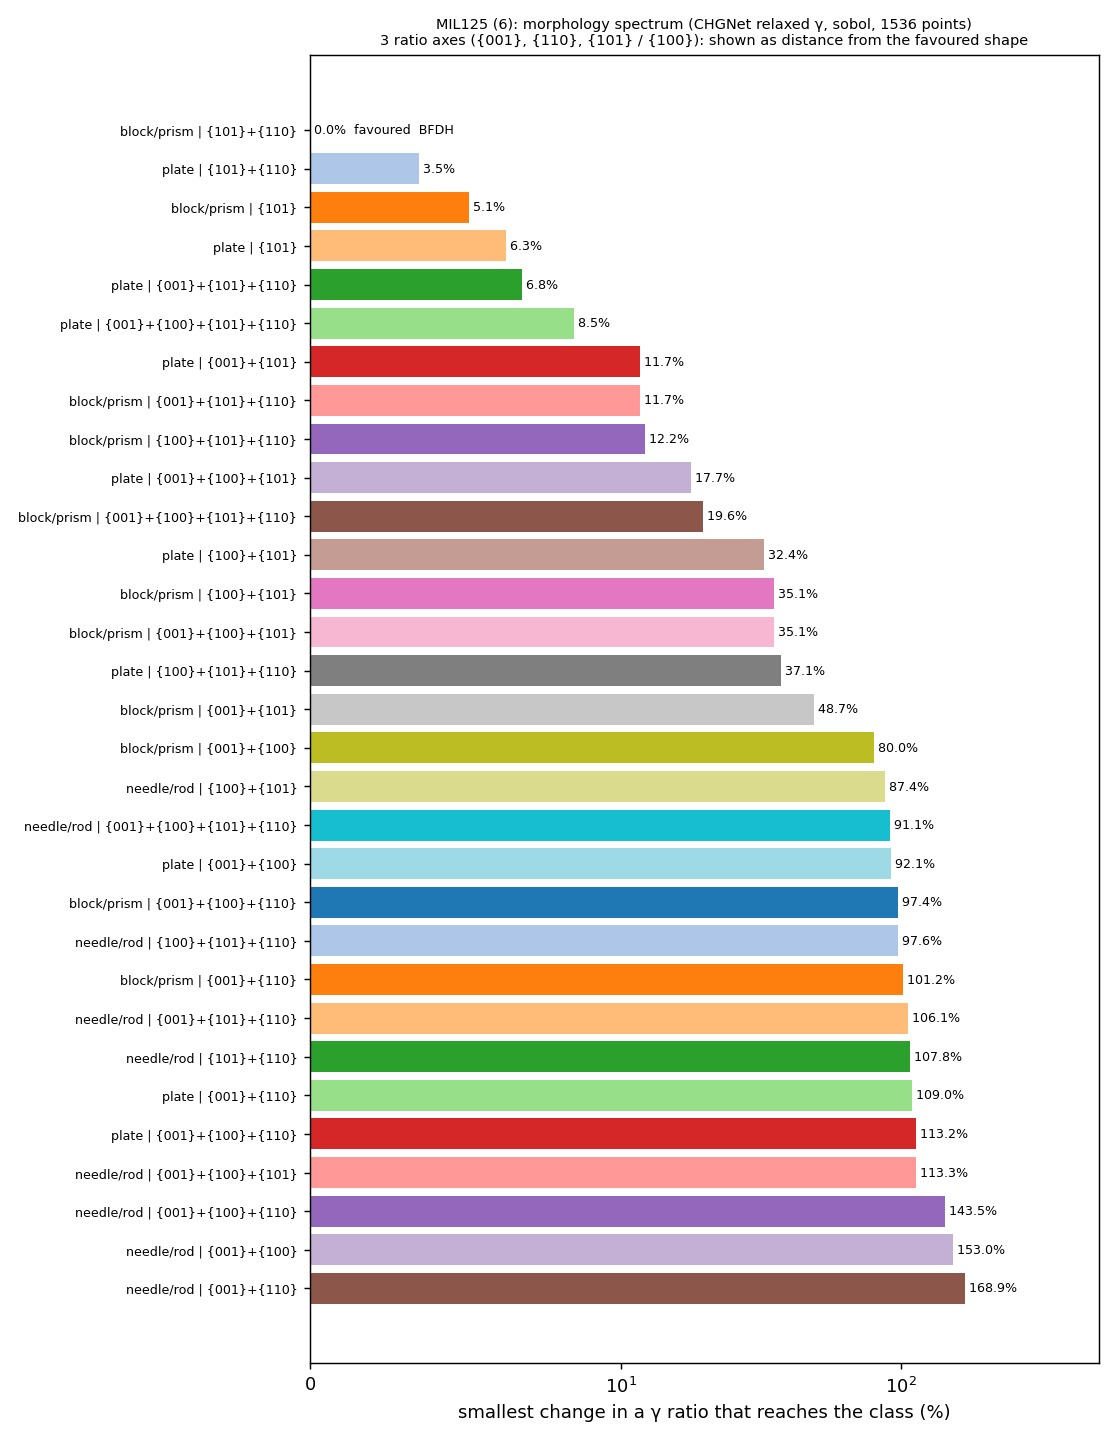
\includegraphics[width=\textwidth]{MIL125_11.jpeg}\\{\tiny CHGNet $\gamma$: classes sorted by distance}
    \end{minipage}\hfill
    \begin{minipage}{0.68\textwidth}\centering
        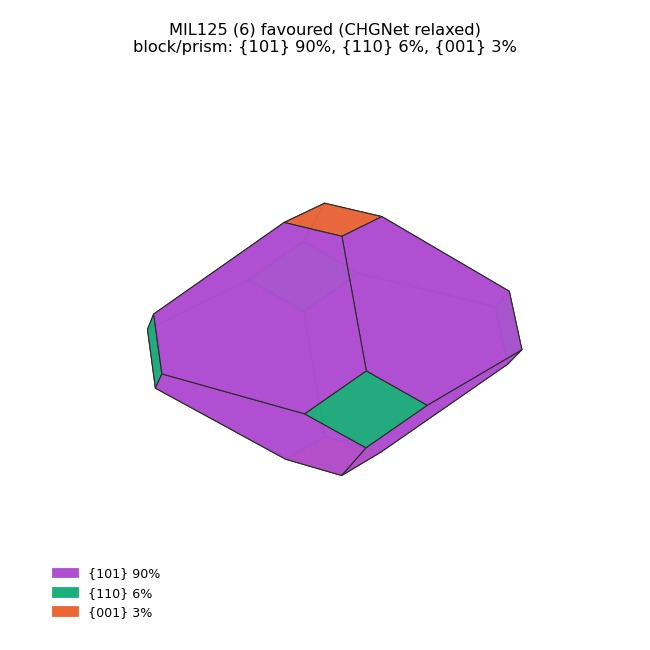
\includegraphics[width=0.32\textwidth]{MIL125_21.jpeg}\hfill
        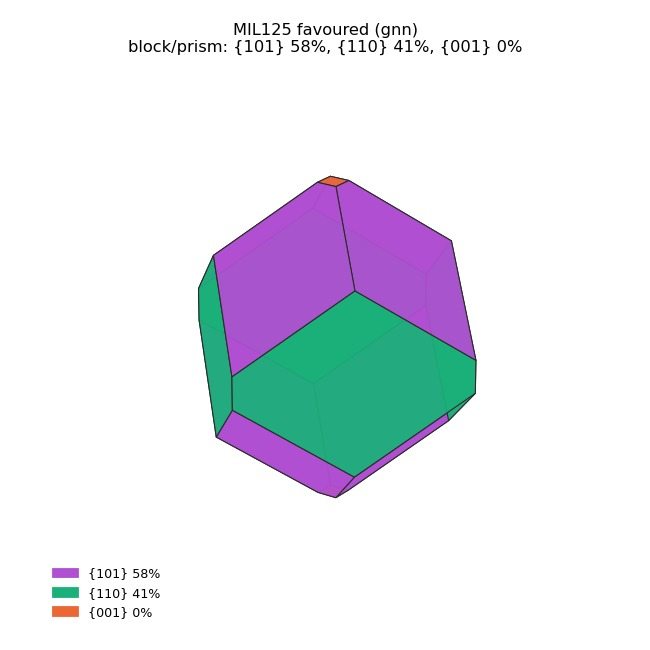
\includegraphics[width=0.32\textwidth]{MIL125_02.jpeg}\hfill
        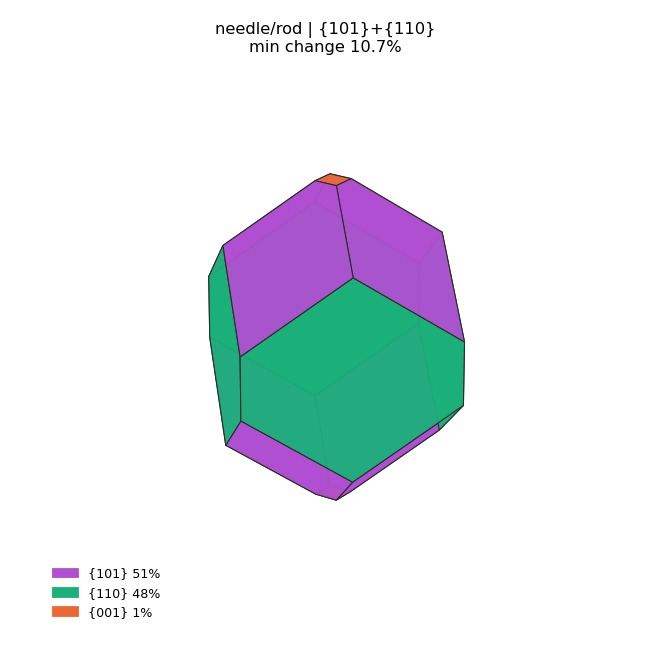
\includegraphics[width=0.32\textwidth]{MIL125_05.jpeg}\\
        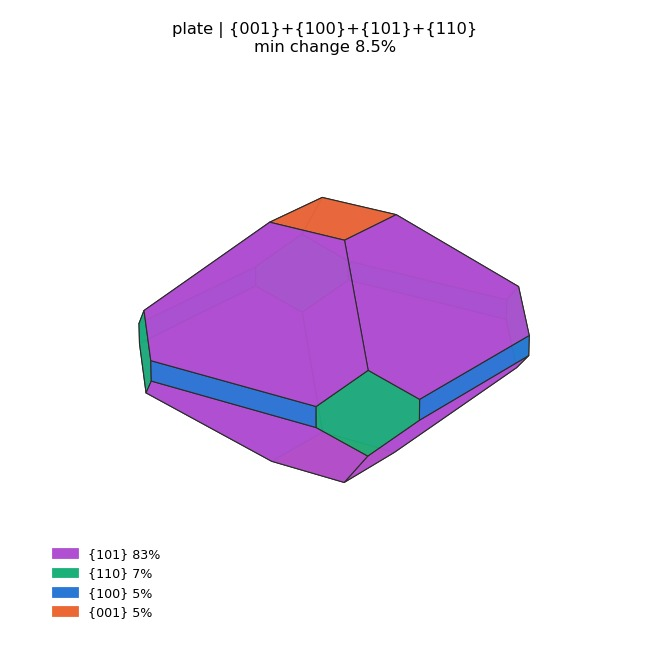
\includegraphics[width=0.32\textwidth]{MIL125_16.jpeg}\hfill
        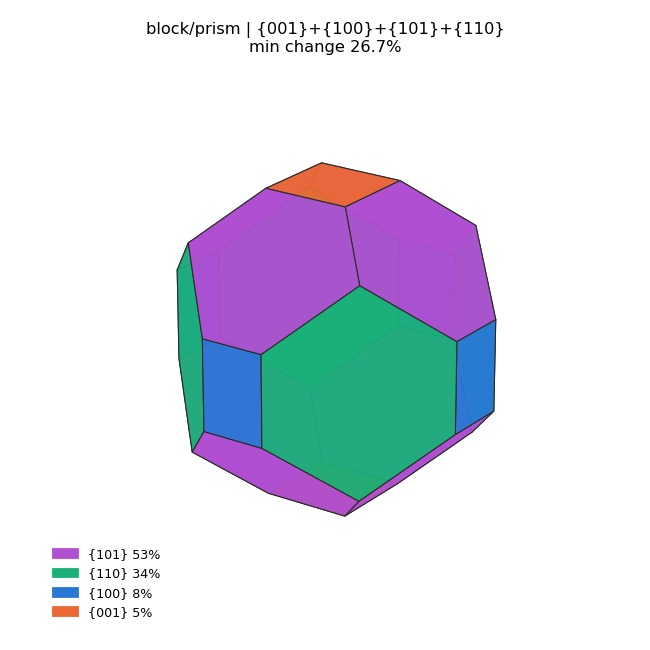
\includegraphics[width=0.32\textwidth]{MIL125_07.jpeg}\hfill
        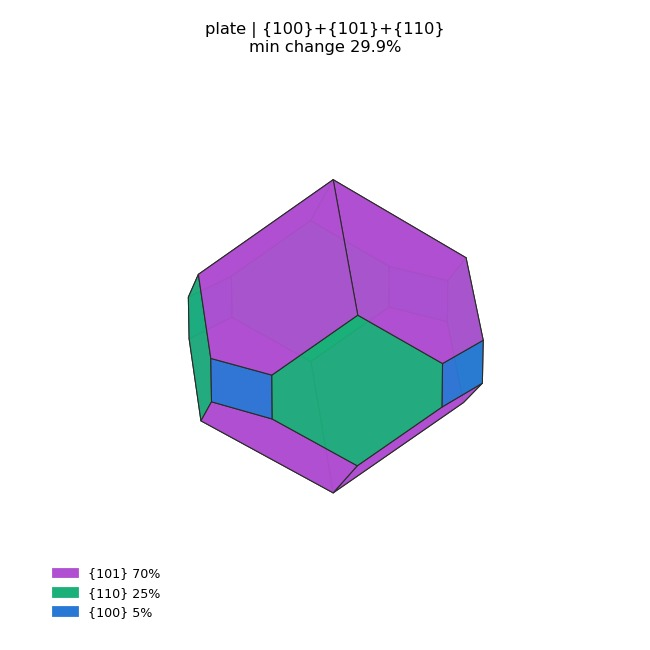
\includegraphics[width=0.32\textwidth]{MIL125_08.jpeg}
    \end{minipage}\\[0.05cm]
    \scriptsize Tetragonal, four faces $\Rightarrow$ 3-axis Sobol scan, 31 classes. Favoured (CHGNet): block, \{101\} 90\%; (GNN): block, \{101\} 58\%, \{110\} 41\%, same class as BFDH. Nearest: plate 3.5\% (CHGNet), rod 10.7\% (GNN). CHGNet values use v4's 0\,K water reference.
\end{frame}

% =========================================================================
% SECTION 4: TECHNICAL KNOWLEDGE
% =========================================================================
\section{Technical Knowledge}

\begin{frame}[shrink=5]{7. Technical Justification, Design Trade-offs \& Insights}
    \framesubtitle{Methodological Rationale \& Design Trade-offs}
    \scriptsize
    \begin{block}{1. Methodological Justification}
        \begin{itemize}
            \item \textbf{Symmetry first:} absences are exact and cost nothing; they remove faces before any energy is computed and already fix ZIF-8's habit.
            \item \textbf{Wulff with stated thermodynamics:} capped surfaces are open systems; the water term must be a chemical potential \cite{reuter2001} with a stated condition, or $\gamma$ can turn negative.
            \item \textbf{Block-intact cuts:} MOFs grow by whole clusters and linkers; cutting a linker leaves radicals never seen in synthesis.
            \item \textbf{Spectrum distances:} for a cubic crystal the class list follows from symmetry; the distance to each class is the structure-specific number and tells how much an additive must change an energy ratio.
        \end{itemize}
    \end{block}
    \begin{block}{2. Design \& Parameter Trade-offs}
        \begin{itemize}
            \item \textbf{CHGNet vs DFT:} 200--600-atom slabs, tens per MOF: DFT needs HPC days, CHGNet minutes; relaxation lowers $\gamma$ by 60--100\%, so values are relative only.
            \item \textbf{Search limits:} \texttt{max\_index} 1 and top-$K$ = 2 relaxations keep runtime practical; high-index faces cannot appear.
            \item \textbf{GNN vs baselines:} kept because it is fast; reported honestly where a one-line model wins.
        \end{itemize}
    \end{block}
\end{frame}

\begin{frame}[shrink=4]{7. Technical Justification, Design Trade-offs \& Insights (contd.)}
    \framesubtitle{Boundary Conditions, Limitations \& Future Scope}
    \scriptsize
    \begin{block}{3. Boundary Conditions \& Edge Cases}
        \begin{itemize}
            \item \textbf{P1 files:} 71 of 77 hMOF CIFs carry no symmetry; only a triclinic cell can be given.
            \item \textbf{Invalid slabs} (not whole formula units, broken organic bonds, clashing caps) are rejected; open Wulff shapes are named ``open''; $\gamma \le 0$ gives no shape rather than a wrong one.
            \item \textbf{Code versions:} the final team notebook (v4) keeps the 0\,K water reference of 14 Nov; the energies reported here come from the corrected run. Isha's spectrum code passes all 20 of its checks with either set of modules.
        \end{itemize}
    \end{block}
    \begin{block}{4. Limitations \& Future Scope}
        \begin{itemize}
            \item \textbf{Not validated:} no $\gamma$ checked by DFT (CP2K inputs ready); UiO-66 additive-free cubes not reproduced; laboratory records and proofs need a second-person check.
            \item \textbf{Equilibrium vs growth:} laboratory crystals are shaped by growth rates and additives; Wulff is a baseline.
            \item \textbf{Next:} DFT on one slab per MOF; caps for modulators (formate, benzoate) at their own chemical potential, read through the spectrum distances; part I (connectivity spectrum $\Delta\alpha$) is closed as a negative result (tracks graph size).
        \end{itemize}
    \end{block}
\end{frame}

% =========================================================================
% REFERENCES & THANK YOU
% =========================================================================
\section{References}
\nocite{wulff1901,donnay1937,grimbergen1998,chgnet2023,mace2024,deng2024softening,core2019,pymatgen2013,spglib2024,tran2016,rappe1992,chen2020,umemura2011,wilmer2012,reuter2001,janaf1998,gilmer2017,sobol1967}
\begin{frame}[allowframebreaks]{References}
    \scriptsize
    \bibliographystyle{ieeetr}
    \bibliography{ref}
\end{frame}

\begin{frame}
    \centering
    {\Huge \textbf{\textcolor{amritaMaroon}{Thank You}}} \\[0.4cm]
    {\large \textbf{Questions \& Viva Voce}}
\end{frame}

\end{document}
